\documentclass{article}
\usepackage{a4wide}
\usepackage[english]{babel}
\usepackage{amsmath}
\usepackage{amssymb}
\usepackage{dsfont}
%\usepackage[dvips]{epsfig}
%\usepackage{graphicx}
\usepackage{fancyhdr}
\usepackage{listings}
\usepackage{nomencl}
\usepackage[pdftex]{graphicx}

\usepackage{listings} 
\lstset{numbers=left, numberstyle=\tiny, numbersep=5pt} 
\lstset{language=C} 
 \lstset{basicstyle=\small}

\pagestyle{fancy}
\lhead{\footnotesize \parbox{11cm}{Andreas Johann H\"ormer (753179), Daniel Tormoen (753148)}}
\rhead{\footnotesize {TMA 4280 Assignment 6}}

\title{Report Assignment 6}
\author{Andreas Johann H\"ormer, Daniel Tormoen}
\date{\today}

\begin{document}
\thispagestyle{empty}
\maketitle
\thispagestyle{empty}
%\\[5cm]
\begin{center}
TMA4280 Supercomputing\\[3cm]
Lab group:
\begin{itemize}
\item Andreas Johann H\"ormer
\item Daniel Tormoen\\[3cm]
\end{itemize}
Report delivered: 27.02.2014\\[6cm]
FACULTY OF INFORMATION TECHNOLOGY, MATHEMATICS AND ELECTRICAL ENGINEERING\\
NORWEGIAN UNIVERSITY OF SCIENCE AND TECHNOLOGY
\end{center}
\thispagestyle{empty}
\newpage
\tableofcontents
\thispagestyle{empty}
\newpage
\section*{Summary}
\thispagestyle{empty}
Matrix dimensions can get very large, so the number of matrix elements can increase quickly. So working with matrices is a perfect way to use distributed computing. In this task the matrix is transposed in the distributed system using MPI. The problem solved is a two dimensional poisson problem. The solution is done for rectangular matrices with homogeneous boundaries. As solution method diagonalization with FST is used.
\newpage
\setcounter{page}{1}
\section{Problem description}
The implementation shall solve the two-dimensional poisson problem 
\begin{equation}
-\bigtriangledown^2=f\;in\;\Omega = (0,1)x(0,1)
\end{equation}
\begin{equation}
u = 0\;on\;\delta\Omega
\end{equation}
The given poisson equation is an elliptic partial differential equation. The problem is solving this equation with given boundary conditions. 
The problem should be discretized with (n+1) points in each spatial direction. The standard 5-point-stencil to discretize the Laplace operator $\bigtriangledown$ has to be used. To obtain a solution in $O(n\cdot log(n))$ the DST should be applied.
\section{Solution strategies}
\subsection{LU factorization}
LU (lower upper) factorization decomposes a matrix in an upper and a lower triangular matrix. This can be done using Gaussian elimination. For symmetric matrizes this can also be done using the cholesky decomposition. The matrix decomposition follows following rule
\begin{equation}
A=LU
\end{equation}
where A is the original matrix, L the lower triangular matrix and U the upper triangular matrix.\\
This solution strategy is not very usable as solver in parallel contexts. The sequential nature (pivoting, substitution, ...) makes it hard for parralelization. The LU factorization needs $\mathcal{O}(n^4)$ for runtime and $\mathcal{O}(n^3)$ for memory when the matrix is sparsed, as well as $\mathcal{O}(n^6)$ Operations and $\mathcal{O}(n^4)$ memory when the matrix is full.
%Runtime O(n^4) sparsed, O(n^6) full
%Memory O(n^3) sparsed, O(n^4) full
\subsection{diagonalization}
The diagonalization can be done in three steps:
\begin{enumerate}
\item $$\underline{\tilde{B}}=\underline{Q^T}\cdot\underline{B}\cdot\underline{Q}$$
\item $$\tilde{x_{ij}}=\frac{\tilde{b_{ij}}}{\lambda_i+\lambda_j}\;for\;1\leq i,j \leq N$$
\item $$\underline{X}=\underline{Q}\cdot\underline{\tilde{X}}\cdot\underline{Q^T}$$
\end{enumerate}
This algorithm scales very well with the number of unknowns and also scales very well in memory. It is better parallelizable than LU factorization. In an further step fourier transform (DST) can be applied. The algorithm has $\mathcal{O}(n^3)$ operations and needs $\mathcal{O}(n^2)$ memory.
%O(n^3) operations
%O(n^2) memory
\subsubsection{diagonalization using DST}
For this diagonalization technique a periodic function with period $2\pi$ is sampled at equidistant points. The function has to be odd and discretized on a equidistant mesh between 0 and $\pi$.The diagonalization can be done in the three following steps:
\begin{enumerate}
\item $$ \underline{\tilde{B}^T}=\underline{S^{-1}}\cdot\big((\underline{S}\cdot\underline{B})^T\big)$$
\item $$ \tilde{x_{ij}}=\frac{\tilde{b_{ij}}}{\lambda_i+\lambda_j}\;for\;1\leq i,j\leq N$$
\item $$ \underline{X}=\underline{S^{-1}}\cdot\big(\underline{S}\cdot(\underline{\tilde{X^T}})\big)^T$$
\end{enumerate}
The diagonalization with discrete sine transform uses $\mathcal{O}(n^2\cdot log(n))$ runtime and needs $\mathcal{O}(n^2)$ memory..

\section{Implemented solution}
	To be able to solve the problem our solution had to be able to evenly divide work among all of the processors and be able to pass that data in a simple way between processors. To solve both of these problems we divided the matrix up so that each processes has a roughly even share of columns in the matrix. Assume $P$ is the number of processes and $n$ is the problem size. We gave $P - (n \bmod P)$ processes $\lfloor (n-1)/P \rfloor$ columns and the rest $\lfloor (n-1)/P \rfloor + 1$ columns. This does not split the data completely evenly, but it makes applying the FST operator more efficient since it operates on a whole column and transpose easier because the data each process sends is always consistent. Different processes only have to communicate to implement the matrix transpose function.

\subsection{Matrix Transpose}
	The matrix is transposed using the message passing interface. This is done using MPI\_Alltoallv(). A code sample for doing this can be seen in section \ref{matrixtranspose}. Each process knows the number of columns in each other process. We must send each other processes as many rows in the sending matrix as the receiving matrix has columns. To do this we reorder the column major data in each process into a row major form to make sending data easier. This makes it so the data that will be sent to each process is located sequentially and we can complete the transpose with only one call to MPI\_Alltoallv(). Once each process receives this data it must be transformed to column major form once again.

\subsection{Parallel FST}
	We parallelized FST using OpenMP. In section \ref{sub:fst} we show the code apply the FST function on each column of $b$. The Fortran code needs to be given a preallocated buffer so we also declare a thread-private buffer $z$ that can be reused each time we call FST or inverse FST in an OpenMP parallel for loop without having to worry about two threads reusing the same buffer. The inverse FST function is implemented in the same way.

\subsection{Proof of Correctness}

	\begin{figure}[htbp]
	\begin{center}
	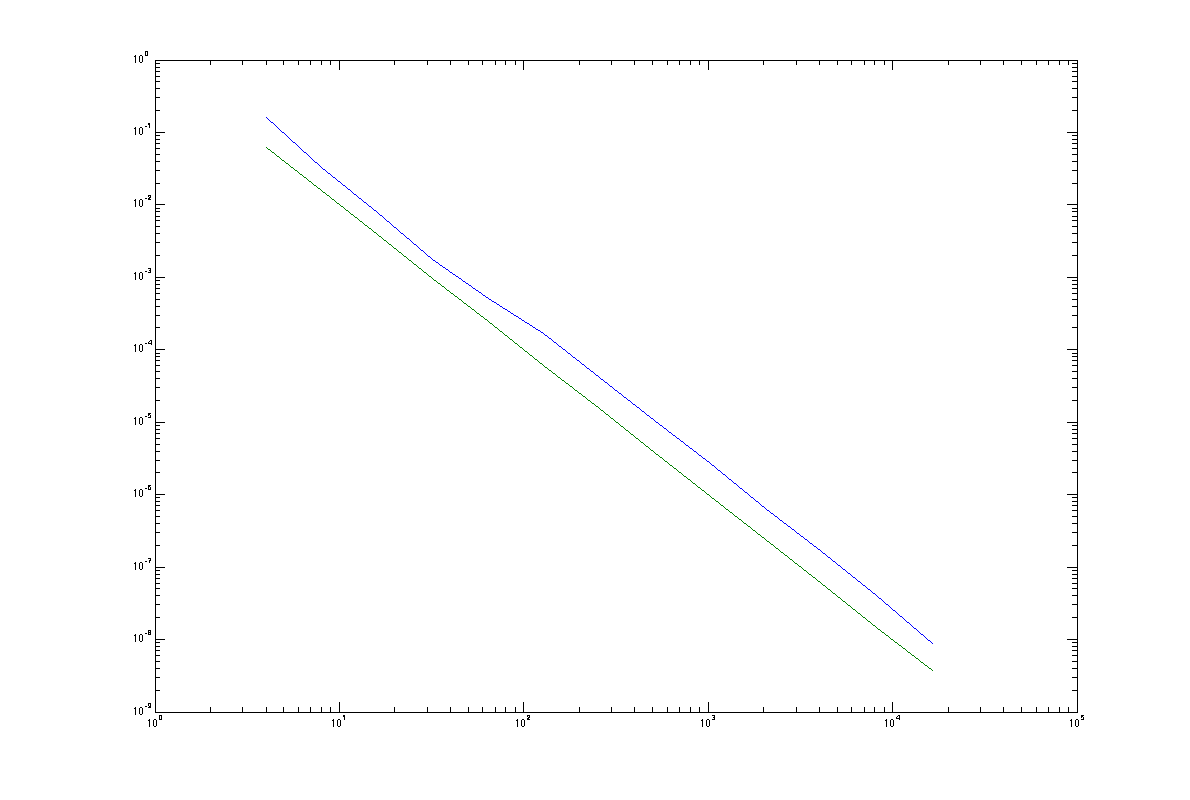
\includegraphics[width=15cm,keepaspectratio=true]{figs/errorGraph}
	\caption{The error decreases as expected.}
	\label{fig:errorGraph}
	\end{center}
	\end{figure}

	To verify the correctness of our method we used a series of tests to ensure each part of the algorithm is producing the results we expect. When we completed the transpose function we tested the transpose function for a variety of sizes and number of MPI processes to ensure that the function was producing the correct matrix. 

	Before we started work on the OpenMP parallelization we tried the complete algorithm with our own function that we knew the exact solution to. We then compared the numeric estimate our program produces to the exact solution to see if they converge. The initial values in each grid location are given by equation \ref{eqn:gridInitial}.

	\begin{equation}
		\label{eqn:gridInitial}
		f(x,y) = 5\pi^2 \sin(\pi x)* \sin(2\pi y)
	\end{equation}

	Equation \ref{eqn:gridExact} shows the exact solution for a grid point. We can find the maximum error at each grid point by taking the absolute value of the difference between the estimate for the grid point and the exact solution. We keep track of the maximum error for any grid point as a measurement of the error.

	\begin{equation}
		\label{eqn:gridExact}
		u(x,y) = \sin(\pi x) * \sin(2 \pi y)
	\end{equation}

	Using this method the maximum error should decrease by a factor of 4 every time we increase the number of grid points in a row by a factor of 2. Assume $e$ is the maximum error for a poisson numerical estimation of size $n \times n$. The error $e$ is given by \ref{eqn:error}.

	\begin{equation}
		\label{eqn:error}
		e = \Theta(\frac{1}{n^2})
	\end{equation}

	We plot our error against this expected error in Figure~\ref{fig:errorGraph}. We generated this graph using the formula from \ref{eqn:error} and by running our program 10 times for each problem size. In each run we found the maximum error in any grid location and found the average max error over the 10 runs. The two lines are parallel so they must only differ by a constant factor. This is the result we predicted so the program must be correct.

\section{Environment}
\subsection{Supercomputer}
The used Kongull cluster is a CentOS 5.3 Linux cluster. The cluster has 1 login, 4 I/O and 93 compute nodes. Each node is equipped with 2x 6-core processors, with 6x 512KiB L1 cache and a common 6 MiB L3-cache. Kongull has 96 compute nodes and 1152 cores in total. All of the compute nodes are HP DL165 G6 servers, with
\begin{itemize}
\item 2 AMD Opteron model 2431 6-core (Istanbul) processors
\item 2.4 GHz core speed
\item 667 MHz (48 GiB nodes) or 800 MHz (24 GiB nodes) bus frequency
\item 149GiB 15000 RPM SAS system disc
\end{itemize}
This and further information about the used supercomputer can be found at the NTNU HPC homepage\footnote{https://www.hpc.ntnu.no/display/hpc/Kongull+Hardware, accessed: 18.03.2014}.
\subsection{Compiler}

For our solution we used following packages on kongull:
\begin{itemize}
\item intelcomp13.0.1
\item openmpi1.4.3-intel
\end{itemize}
\section{Results}

	\begin{figure}[htbp]
	\begin{center}
	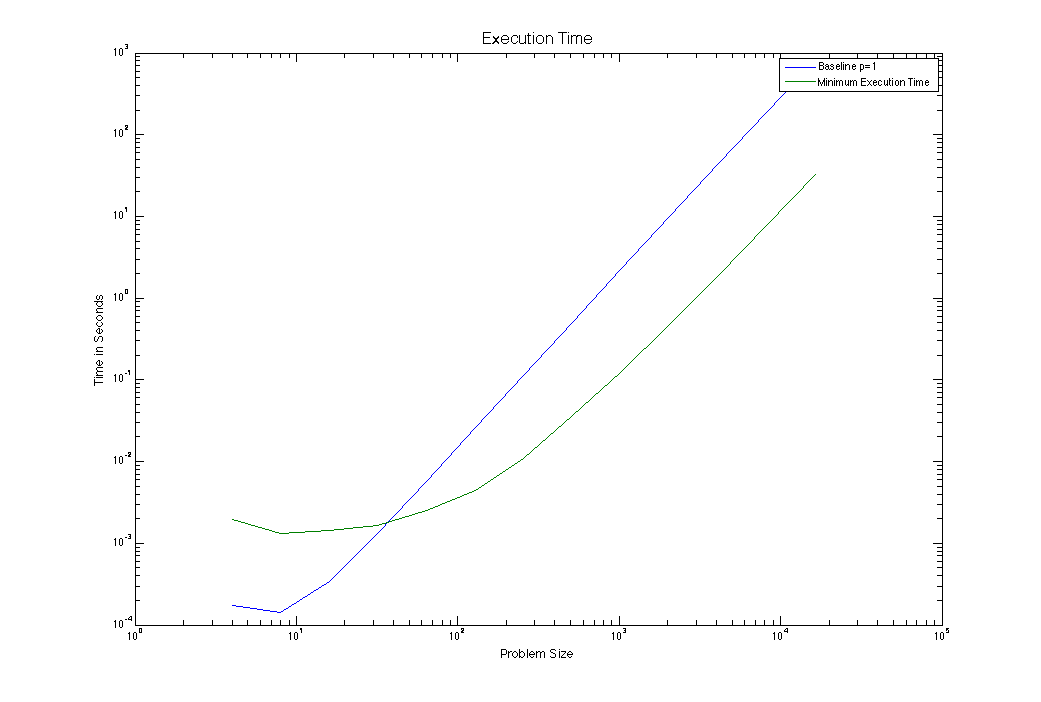
\includegraphics[width=15cm,keepaspectratio=true]{figs/executionTime}
	\caption{The minimum execution time of each problem size. See Figure~\ref{fig:threadsProcesses} for a graph of the number of OpenMP threads and MPI processes that were used to achieve the minimum execution times.}
	\label{fig:executionTime}
	\end{center}
	\end{figure}

\subsection{Execution Times}

	Figure~\ref{fig:executionTime} compares the time the fastest parallelized version where $p=36$ with the baseline $p=1$. Using 36 processors has some overhead to synchronize the processors and share data so for small problem sizes the execution time is slower. As the problem size grows, this overhead become very small compared to the processing required to solve the poisson problem, so using 36 processors performs much better. The point where using 36 processors becomes faster than a single processor is very close to $n=36$. This represents the point where the time saved in overhead to coordinate 36 processors is equal to the time saved being able to processes data faster. When $n$ is sufficiently large, both the single processor and 36 processor version experience exponential growth in execution time.  

	\begin{figure}[htbp]
	\begin{center}
	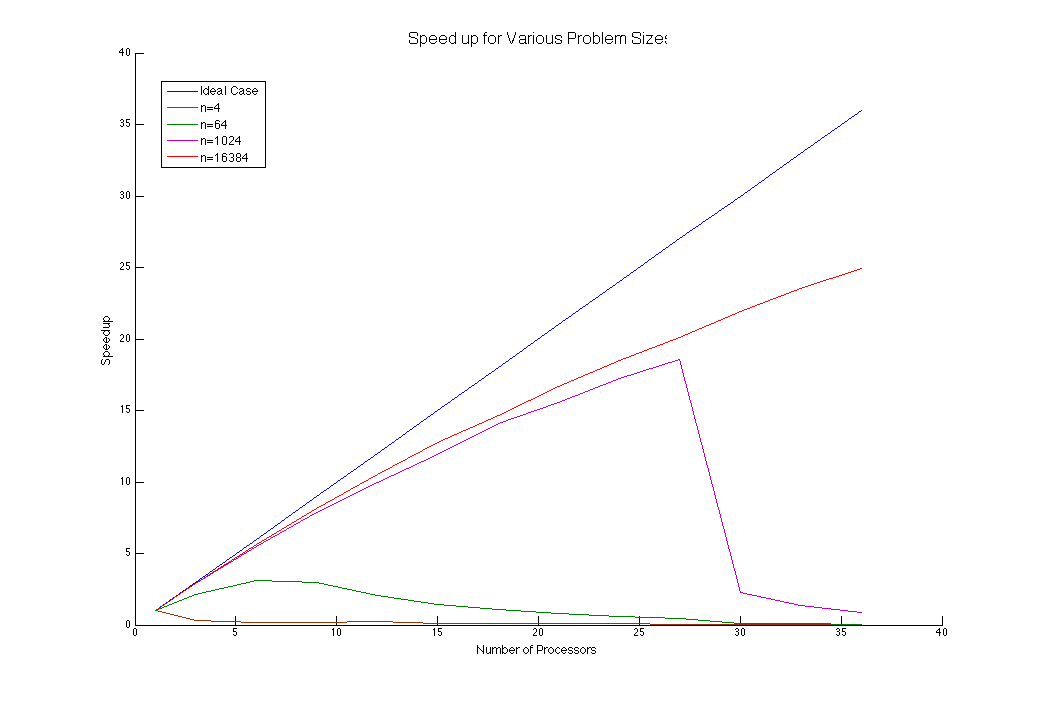
\includegraphics[width=15cm,keepaspectratio=true]{figs/speedup}
	\caption{The speed up for a selection of problem sizes compared to the ideal speed up. There appears to be an ideal number of processors for each problem size where the speed up is the highest. This was run on Kongull using purely MPI.}
	\label{fig:speedup}
	\end{center}
	\end{figure}

\subsection{Speedup} \label{sub:speedup}

	Figure~\ref{fig:speedup} shows the speed up for $n=4,64,1024,16384$ and the ideal case for processors $p=3,6,9,...,36$. We generated this graph by averaging the speedup after running our code 5 times on Kongull. For $n=4$ parallelizing the code actually results in a decrease in speed. The problem size is so small that the overhead of coordinating multiple processes is far more than the gains from parallelizing it. Because we are dividing the matrix into columns if we have more than 3 processes some will not actually have any work to do. The other problem sizes shown all get some speedup for parallelization, but there appears to be a size where there is no longer any gains. $n=64$ peaks at 6 processes and at around 15 processors starts to have a speed up less than 1. $n=1024$ peaks at 27 processors. We do not see the peak for $n=16384$, but there is diminishing returns for each processor.


	

\section{Analysis}

\subsection{Memory Usage}

	For our analysis we will us $M$ as the number of MPI processes, $T$ as the number of OpenMP threads, and $n$ as the problem size. We generate a matrix as well as allocate storage for the transpose matrix of size $\Theta(n^2)$. These matrices are split across all of the processes so each process contains $\Theta(\frac{n^2}{M})$. The diagonal matrix requires $\Theta(n)$ and is stored on each process. To store the information for the transpose function we generate $2M$ arrays each of size $\Theta(M)$, 2 for each process. These store the size of each process and the data offsets. We also must create a buffer of size $\Theta(n)$ for each OpenMP thread to pass to the FST function for temporary values. Therefore the overall memory usage is:

	\begin{equation}
		\Theta(n^2) + \Theta(nM) + \Theta(M^2) + \Theta(nT)
	\end{equation}

	As our results in section~\ref{sub:speedup} show the speed up is much worse when the number of processors used is larger than the problem size. Therefore in any practical example $\Theta(n^2) > \Theta(M^2)$, $\Theta(n^2) > \Theta(nM)$, and $\Theta(n^2) > \Theta(nT)$. In any case where there is a speed up greater than 1 the memory usage of our program is $\Theta(n^2)$.

	\begin{figure}[htbp]
	\begin{center}
	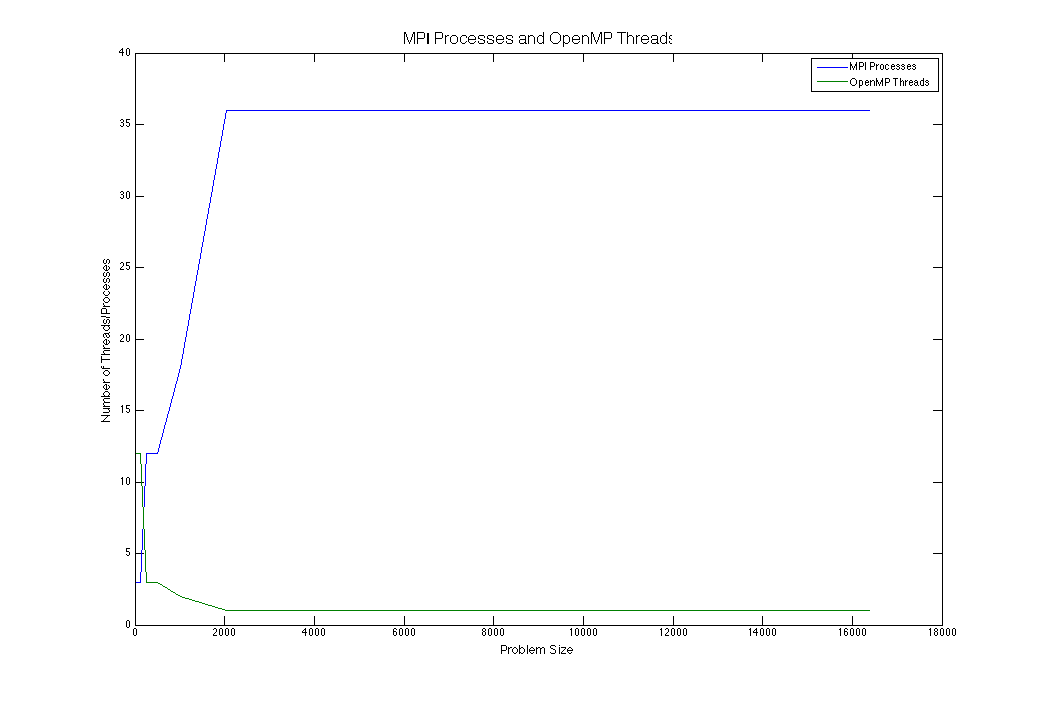
\includegraphics[width=15cm,keepaspectratio=true]{figs/threadsProcesses}
	\caption{The number MPI processes and OpenMP threads per process that produced the minimum execution time for each problem size. When the problem size is sufficiently large, using purely MPI produces the fastest results.}
	\label{fig:threadsProcesses}
	\end{center}
	\end{figure}

\subsection{OpenMP, MPI, or Hybrid}

	In Figure~\ref{fig:threadsProcesses} we can see that for larger problem sizes, using mostly or completely MPI results in faster execution times. The main reason for this is that when we increase the number of MPI processes we are increasing the parallelization of both the FST steps and the transpose step. When we increase the number of OpenMP threads we are only parallelizing the FST step. When there are more MPI processes each process has to send and receive a much smaller piece of data than if there are more OpenMP threads. Different processes can independently send and receive data so when we have more MPI processes more data can be sent and received concurrently. For smaller problem sizes the overhead of synchronizing many processes is too high so favoring OpenMP threads is more efficient. A relatively small amount of data has to be transferred so the transpose step is much faster with fewer processes.


%\begin{figure}[htbp]
%\begin{center}
%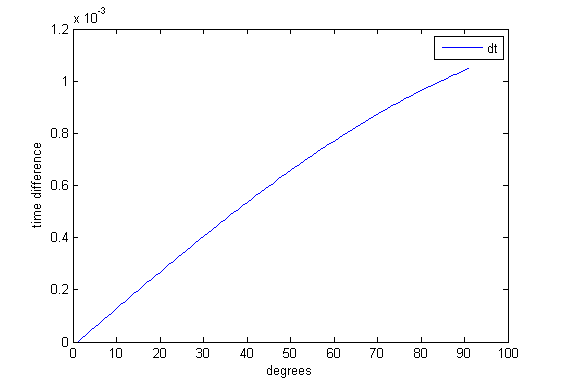
\includegraphics[width=15cm,keepaspectratio=true]{angles}
%\caption{Time differences for sound signal at two ears}
%\label{fig:angles}
%\end{center}
%\end{figure}



\section{Possible optimizations}
\subsection{parallel FST}
In our algorithm the FST is serial. This could be a possible bottleneck. Parallelizing this FST-algorithm may increase the performance.
\subsection{rectangular matrix}
Our algorithm is designed for handling squared matrices with zero-boundary. For handling rectangular matrices this can be done with following:
\begin{equation}
-U_0+2U_1-U_2=h^2f_1
\end{equation}
When moving $U_0$ to the other side and writing in a general form this changes to
\begin{equation}
-U_{N-2}+2U_{N-1}-U_N=h^2f_{N-1}
\end{equation}
For rectangular matrices the sizing in x- and y-direction is different. So the multiplication is done with two different variables, $h_x$ and $h_y$.
\begin{equation}
\frac{1}{h_x^2}A_DU+\frac{1}{h_y^2}UA_D=F
\end{equation}
The matrix which is added on the right side looks then
$$
\begin{bmatrix}
U_{1,1} & U_{2,1} & 0 & ... & 0 & U_{N_x-1,1} & U_{N_x,1} \\
U_{1,2} & 0 & ... & ... & ... & 0 & U_{N_x,2} \\
... & ... & ... & ... &... & ... & ... \\
U_{1,N_y} & U_{2,N_y} & 0 & ... & 0 & U_{N_x-1,N_y} & U_{N_x,N_y} 
\end{bmatrix}
$$
\subsection{non-homogeneous boundary conditions}
This optimization can be done in a similar way to the rectangular matrices. The boundary has to be moved to the right side which looks like the rectangular matrix. The calculation can be done using following formula
\begin{equation}
\frac{G_{i,j}}{\frac{1}{\sqrt{h_x^2}}\lambda_i+\frac{1}{\sqrt{h_x^2}}\lambda_j}
\end{equation}
%parallel fst
%not much possibilities
\newpage
\section{Conclusion}
In this exercise an implementation of a two dimensional poisson solver was done. The method used is diagonalization using FST with a runtime of $\mathcal{O}(n^2\cdot log(n))$. The algorithm is parallelized in such a way that the transpose of the matrix is distributed using MPI. The implemented algorithm is considered to use squared matrices with homogeneous borders. A theoretical analysis of a way how to change the algorithm to use rectangular and non-homogeneous matrices was done.

\section{Appendix}
\subsection{Git Repository}
	The latest version of the source code can be found in a git repository\footnote{https://github.com/Horn2BWild/NTNU2014/tree/supercomp\_ex6/TMA4280\_Supercomputing/Exercise/ex6}.

\subsection{Code samples}
\subsubsection{Matrix transpose\label{matrixtranspose}}
\begin{lstlisting}[caption=Matrix transposition using MPI]{Matrix transpose}
for(rowcnt=0; rowcnt<m; rowcnt++)
{
    for(columncnt=0; columncnt<scnt[rank]; columncnt++)
    {
        sendvector[vectorposition]=b[columncnt][rowcnt];
        vectorposition++;
    }
}
MPI_Alltoallv (
    sendvector, MPIscnt, MPIdispl, MPI_DOUBLE, receivevector,
    MPIscnt, MPIdispl, MPI_DOUBLE, MPI_COMM_WORLD);
for (proccnt = 0; proccnt < size; ++proccnt)
{
    for(columncnt=0; columncnt<scnt[rank];columncnt++)
    {
        for (rowcnt = displ[proccnt]; 
        	rowcnt < displ[proccnt] + scnt[proccnt]; ++rowcnt)
        {

            bt[columncnt][rowcnt]=receivevector[vectorposition];
            vectorposition++;
        }
    }
}
\end{lstlisting}
Description:
\begin{itemize}
\item line 1-8: generating send vector from matrix
\item line 9-11: send and receive vector to/from distributed system\\
For this MPI\_Alltoallv() was used. This function splits the data from each process over each of the processes so that after the call each process has the information needed to complete the transpose, although it is not in column major form.
\item line 12-24: generating transposed matrix from received vector
\end{itemize}

\subsubsection{FST Parallelization \label{sub:fst}}
\begin{lstlisting}[caption=Parallelizing the FST function]{FST}
int nn = 4*n;
static Real *z;
#pragma omp threadprivate(z)
#pragma omp parallel
    {
        z = createRealArray (nn);
    }
#pragma omp parallel for schedule(guided,1)
    for (j=0; j < scnt[rank]; j++)
    {
        fst_(b[j], &n, z, &nn);
    }
\end{lstlisting}

\end{document}
